\documentclass[10pt,fleqn]{article} % Default font size and left-justified equations
\usepackage[%
    pdftitle={Modélisation SLCI : Rapidité des systèmes},
    pdfauthor={Xavier Pessoles}]{hyperref}
    
%%%%%%%%%%%%%%%%%%%%%%%%%%%%%%%%%%%%%%%%%
% Original author:
% Mathias Legrand (legrand.mathias@gmail.com) with modifications by:
% Vel (vel@latextemplates.com)
% License:
% CC BY-NC-SA 3.0 (http://creativecommons.org/licenses/by-nc-sa/3.0/)
%%%%%%%%%%%%%%%%%%%%%%%%%%%%%%%%%%%%%%%%%

%----------------------------------------------------------------------------------------
%	VARIOUS REQUIRED PACKAGES AND CONFIGURATIONS
%----------------------------------------------------------------------------------------

%\usepackage[top=2.5cm,bottom=2cm,left=2cm,right=2cm,headsep=40pt,a4paper]{geometry} % Page margins
\usepackage[top=2cm,bottom=3cm,left=2cm,right=2cm,a4paper]{geometry} % Page margins

\usepackage{graphicx} % Required for including pictures

\usepackage{lipsum} % Inserts dummy text

\usepackage{tikz} % Required for drawing custom shapes

\usepackage[francais]{babel} % English language/hyphenation
\frenchbsetup{StandardLists=true} % Pour éviter la collision babel enumitem pour les listes

\usepackage{enumitem} % Customize lists
\setlist{nolistsep} % Reduce spacing between bullet points and numbered lists

\usepackage{booktabs} % Required for nicer horizontal rules in tables

\usepackage{xcolor} % Required for specifying colors by name
%\definecolor{ocre}{RGB}{243,102,25} % Define the orange color used for highlighting throughout the book
 \definecolor{ocre}{RGB}{49,133,156} % Couleur ''bleue''
\definecolor{violetf}{RGB}{112,48,160} % Couleur ''violet''
\usepackage{enumitem}
\usepackage{pifont} % Pour les dinglist
\usepackage{multicol}
\usepackage{array} % Centrage vertical dans les tableaux

%----------------------------------------------------------------------------------------
%	FONTS
%----------------------------------------------------------------------------------------

\usepackage{multicol}
\usepackage{siunitx}
\sisetup{output-decimal-marker = {,}}


\usepackage{avant} % Use the Avantgarde font for headings
%\usepackage{times} % Use the Times font for headings
%\usepackage{mathptmx} % Use the Adobe Times Roman as the default text font together with math symbols from the Sym­bol, Chancery and Com­puter Modern fonts
\usepackage[adobe-utopia]{mathdesign}
\usepackage{microtype} % Slightly tweak font spacing for aesthetics
\usepackage[utf8]{inputenc} % Required for including letters with accents
\usepackage[T1]{fontenc} % Use 8-bit encoding that has 256 glyphs

%----------------------------------------------------------------------------------------
%	BIBLIOGRAPHY AND INDEX
%----------------------------------------------------------------------------------------

%\usepackage[style=alphabetic,citestyle=numeric,sorting=nyt,sortcites=true,autopunct=true,babel=hyphen,hyperref=true,abbreviate=false,backref=true,backend=biber]{biblatex}
\usepackage[style=alphabetic,citestyle=numeric,sorting=nyt,sortcites=true,autopunct=true,hyperref=true,abbreviate=false,backref=true,backend=biber]{biblatex}
\addbibresource{bibliography.bib} % BibTeX bibliography file
\defbibheading{bibempty}{}

\usepackage{calc} % For simpler calculation - used for spacing the index letter headings correctly
\usepackage{makeidx} % Required to make an index
\makeindex % Tells LaTeX to create the files required for indexing

%----------------------------------------------------------------------------------------
%	MAIN TABLE OF CONTENTS
%----------------------------------------------------------------------------------------

\usepackage{titletoc} % Required for manipulating the table of contents

\setcounter{tocdepth}{2}     % Dans la table des matieres
\setcounter{secnumdepth}{2}

\contentsmargin{0cm} % Removes the default margin

% Part text styling
\titlecontents{part}[0cm]
{\addvspace{20pt}\centering\large\bfseries}
{}
{}
{}

% Chapter text styling
\titlecontents{chapter}[1.25cm] % Indentation
{\addvspace{12pt}\large\sffamily\bfseries} % Spacing and font options for chapters
{\color{ocre!60}\contentslabel[\Large\thecontentslabel]{1.25cm}\color{ocre}} % Chapter number
{\color{ocre}}  
{\color{ocre!60}\normalsize\;\titlerule*[.5pc]{.}\;\thecontentspage} % Page number

% Section text styling
\titlecontents{section}[1.25cm] % Indentation
{\addvspace{3pt}\sffamily\bfseries} % Spacing and font options for sections
{\color{ocre!60}\contentslabel[\thecontentslabel]{1.25cm} \color{ocre}} % Section number
{\color{ocre}}
{\hfill\color{ocre!60}\thecontentspage} % Page number
[]

% Subsection text styling
\titlecontents{subsection}[1.25cm] % Indentation
{\addvspace{1pt}\sffamily\small} % Spacing and font options for subsections
{\contentslabel[\thecontentslabel]{1.25cm}} % Subsection number
{}
{\ \titlerule*[.5pc]{.}\;\thecontentspage} % Page number
[]


% Subsection text styling
\titlecontents{subsubsection}[1.25cm] % Indentation
{\addvspace{1pt}\sffamily\small} % Spacing and font options for subsections
{\contentslabel[\thecontentslabel]{1.25cm}} % Subsection number
{}
{\ \titlerule*[.5pc]{.}\;\thecontentspage} % Page number
[]

% List of figures
\titlecontents{figure}[0em]
{\addvspace{-5pt}\sffamily}
{\thecontentslabel\hspace*{1em}}
{}
{\ \titlerule*[.5pc]{.}\;\thecontentspage}
[]

% List of tables
\titlecontents{table}[0em]
{\addvspace{-5pt}\sffamily}
{\thecontentslabel\hspace*{1em}}
{}
{\ \titlerule*[.5pc]{.}\;\thecontentspage}
[]

%----------------------------------------------------------------------------------------
%	MINI TABLE OF CONTENTS IN PART HEADS
%----------------------------------------------------------------------------------------

% Chapter text styling
\titlecontents{lchapter}[0em] % Indenting
{\addvspace{15pt}\large\sffamily\bfseries} % Spacing and font options for chapters
{\color{ocre}\contentslabel[\Large\thecontentslabel]{1.25cm}\color{ocre}} % Chapter number
{}  
{\color{ocre}\normalsize\sffamily\bfseries\;\titlerule*[.5pc]{.}\;\thecontentspage} % Page number

% Section text styling
\titlecontents{lsection}[0em] % Indenting
{\sffamily\small} % Spacing and font options for sections
{\contentslabel[\thecontentslabel]{1.25cm}} % Section number
{}
{}

% Subsection text styling
\titlecontents{lsubsection}[.5em] % Indentation
{\normalfont\footnotesize\sffamily} % Font settings
{}
{}
{}

%----------------------------------------------------------------------------------------
%	PAGE HEADERS
%----------------------------------------------------------------------------------------

\usepackage{fancyhdr} % Required for header and footer configuration



\pagestyle{fancy}
 \renewcommand{\headrulewidth}{0pt}
 \fancyhead{}
 
 % ENTETES de page
 \fancyhead[L]{%
 \noindent\begin{minipage}[c]{2.6cm}%
 
\includegraphics[width=2cm]{logo_lycee.png}%
 \end{minipage}}

\fancyhead[C]{\rule{8cm}{.5pt}}

 \fancyhead[R]{%
 \noindent\begin{minipage}[c]{3cm}
 \begin{flushright}
 \footnotesize{\textit{\textsf{\xxtete}}}%
 \end{flushright}
 \end{minipage}
}

 \fancyfoot{}
 % PIEDS de page
\fancyfoot[C]{\rule{12cm}{.5pt}}
\renewcommand{\footrulewidth}{0.2pt}
\fancyfoot[C]{\footnotesize{\bfseries \thepage}}
\fancyfoot[L]{ 
\begin{minipage}[c]{.4\linewidth}
\noindent\footnotesize{{\xxauteur}}
\end{minipage}}

\fancyfoot[R]{\footnotesize{\xxpied}
\ifthenelse{\isodd{\value{page}}}{
\begin{tikzpicture}[overlay]
\node[shape=rectangle, 
      rounded corners = .25 cm,
	  draw= ocre,
	  line width=2pt, 
	  fill = ocre!10,
	  minimum width  = 2.5cm,
	  minimum height = 3cm,] at (\xxposongletx,\xxposonglety) {};
\node at (\xxposonglettext,\xxposonglety) {\rotatebox{90}{\textbf{\large\color{ocre}{\xxonglet}}}};
%{};
\end{tikzpicture}}{}
}



%
%
%
% Removes the header from odd empty pages at the end of chapters
\makeatletter
%\renewcommand{\cleardoublepage}{
%\clearpage\ifodd\c@page\else
%\hbox{}
%\vspace*{\fill}
%\thispagestyle{empty}
%\newpage
%\fi}

%\fancypagestyle{plain}{%
%\fancyhf{} % vide l’en-tête et le pied~de~page.
%%\fancyfoot[C]{\bfseries \thepage} % numéro de la page en cours en gras
%% et centré en pied~de~page.
%\fancyfoot[R]{\footnotesize{\xxpied}}
%\fancyfoot[C]{\rule{12cm}{.5pt}}
%\renewcommand{\footrulewidth}{0.2pt}
%\fancyfoot[C]{\footnotesize{\bfseries \thepage}}
%\fancyfoot[L]{ 
%\begin{minipage}[c]{.4\linewidth}
%\noindent\footnotesize{{\xxauteur}}
%\end{minipage}}}

\fancypagestyle{plain}{%
\fancyhf{} % vide l’en-tête et le pied~de~page.
\fancyfoot[C]{\rule{12cm}{.5pt}}
\renewcommand{\footrulewidth}{0.2pt}
\fancyfoot[C]{\footnotesize{\bfseries \thepage}}
\fancyfoot[L]{ 
\begin{minipage}[c]{.4\linewidth}
\noindent\footnotesize{{\xxauteur}}
\end{minipage}}
\fancyfoot[R]{\footnotesize{\xxpied}}
}



%----------------------------------------------------------------------------------------
%	THEOREM STYLES
%----------------------------------------------------------------------------------------

% Conflit avec la police adobe
%\usepackage{amsmath,amsfonts,amssymb,amsthm} % For math equations, theorems, symbols, etc
\usepackage{amsmath,amsthm}

\newcommand{\intoo}[2]{\mathopen{]}#1\,;#2\mathclose{[}}
\newcommand{\ud}{\mathop{\mathrm{{}d}}\mathopen{}}
\newcommand{\intff}[2]{\mathopen{[}#1\,;#2\mathclose{]}}
%\newtheorem{notation}{Notation}[chapter]
\newtheorem{notation}{Notation}[section]

% Boxed/framed environments
\newtheoremstyle{ocrenumbox}% % Theorem style name
{0pt}% Space above
{0pt}% Space below
{\normalfont}% % Body font
{}% Indent amount
{\small\bf\sffamily\color{ocre}}% % Theorem head font
{\;}% Punctuation after theorem head
{0.25em}% Space after theorem head
{\small\sffamily\color{ocre}\thmname{#1}\nobreakspace\thmnumber%{\@ifnotempty{#1}{}\@upn{#2}}% Theorem text (e.g. Theorem 2.1)
\thmnote{\nobreakspace\the\thm@notefont\sffamily\bfseries\color{black}---\nobreakspace#3.}} % Optional theorem note
\renewcommand{\qedsymbol}{$\blacksquare$}% Optional qed square


% Boite pour les corriges
\newtheoremstyle{correctionbox}% % Theorem style name
{0pt}% Space above
{0pt}% Space below
{\normalfont}% % Body font
{}% Indent amount
{\small\bf\sffamily\color{violet}}% % Theorem head font
{\;}% Punctuation after theorem head
{0.25em}% Space after theorem head
{\small\sffamily\color{ocre}\thmname{#1}\nobreakspace\thmnumber%{\@ifnotempty{#1}{}\@upn{#2}}% Theorem text (e.g. Theorem 2.1)
\thmnote{\nobreakspace\the\thm@notefont\sffamily\bfseries\color{black}---\nobreakspace#3.}} % Optional theorem note
\renewcommand{\qedsymbol}{$\blacksquare$}% Optional qed square



\newtheoremstyle{blacknumex}% Theorem style name
{5pt}% Space above
{5pt}% Space below
{\normalfont}% Body font
{} % Indent amount
{\small\bf\sffamily}% Theorem head font
{\;}% Punctuation after theorem head
{0.25em}% Space after theorem head
{\small\sffamily{\tiny\ensuremath{\blacksquare}}\nobreakspace\thmname{#1}\nobreakspace\thmnumber%{\@ifnotempty{#1}{}\@upn{#2}}% Theorem text (e.g. Theorem 2.1)
\thmnote{\nobreakspace\the\thm@notefont\sffamily\bfseries---\nobreakspace#3.}}% Optional theorem note

\newtheoremstyle{blacknumbox} % Theorem style name
{0pt}% Space above
{0pt}% Space below
{\normalfont}% Body font
{}% Indent amount
{\small\bf\sffamily}% Theorem head font
{\;}% Punctuation after theorem head
{0.25em}% Space after theorem head
{\small\sffamily\thmname{#1}\nobreakspace 
\thmnote{\nobreakspace\the\thm@notefont\sffamily\bfseries---\nobreakspace#3.}}% Optional theorem note

% Non-boxed/non-framed environments
\newtheoremstyle{ocrenum}% % Theorem style name
{5pt}% Space above
{5pt}% Space below
{\normalfont}% % Body font
{}% Indent amount
{\small\bf\sffamily\color{ocre}}% % Theorem head font
{\;}% Punctuation after theorem head
{0.25em}% Space after theorem head
{\small\sffamily\color{ocre}\thmname{#1}\nobreakspace%\thmnumber{\@ifnotempty{#1}{}\@upn{#2}}% Theorem text (e.g. Theorem 2.1)
\thmnote{\nobreakspace\the\thm@notefont\sffamily\bfseries\color{black}---\nobreakspace#3.}} % Optional theorem note
\renewcommand{\qedsymbol}{$\blacksquare$}% Optional qed square
\makeatother

% Environnement pour les titres de parties
\newtheoremstyle{partiebox} 
{0pt}% Space above
{0pt}% Space below
{\normalfont}% Body font
{}% Indent amount
{\small\bf\sffamily}% Theorem head font
{\;}% Punctuation after theorem head
{0.25em}% Space after theorem head




% Defines the theorem text style for each type of theorem to one of the three styles above
\newcounter{dummy} 
\numberwithin{dummy}{section}
\theoremstyle{ocrenumbox}
%\newtheorem{theoremeT}[dummy]{Théorème}
\newtheorem{theoremeT}[dummy]{Théorème}
\newtheorem{resultatT}[dummy]{Résultat}
\newtheorem{savoirT}[dummy]{Savoir}
\newtheorem{methodeT}[dummy]{Méthode}
\newtheorem{objectifT}[dummy]{Objectif}
%\newtheorem{problem}{Problem}[chapter]
\newtheorem{problem}{Problem}[section]
%\newtheorem{exerciseT}{Exercise}[chapter]
\newtheorem{exerciseT}{Exercice}[section]

\theoremstyle{blacknumex}
%\newtheorem{exampleT}{Example}[chapter]
\newtheorem{exempleT}{Exemple}[section]
\newtheorem{termT}{Terminal\\}[section]
\newtheorem{pyT}{Python\\}[section]
\newtheorem{sciT}{Scilab\\}[section]
\newtheorem{pseudoT}{Pseudo Code\\}[section]
\newtheorem{sqlT}{SQL\\}[section]

\theoremstyle{blacknumbox}
%\newtheorem{vocabulary}{Vocabulary}[chapter]
\newtheorem{vocabulary}{Vocabulaire}[section]
%\newtheorem{definitionT}{Definition}[section]
\newtheorem{definitionT}{Définition}[section]
\newtheorem{rappelT}{Rappel}[section]
\newtheorem{demoT}{Démonstration}[section]
\newtheorem{corollaryT}[dummy]{Corollaire}
\newtheorem{hypoT}{Hypothèse(s)}

\theoremstyle{ocrenum}
\newtheorem{proposition}[dummy]{Proposition}

\theoremstyle{partiebox}
\newtheorem{titrepartieT}[]{}
\newtheorem{titrechapitreT}[]{}

\theoremstyle{correctionbox}
\newtheorem{correctionT}[dummy]{\color{violet}{Correction}}

%----------------------------------------------------------------------------------------
%	DEFINITION OF COLORED BOXES
%----------------------------------------------------------------------------------------

\RequirePackage[framemethod=tikz]{mdframed} % Required for creating the theorem, definition, exercise and corollary boxes

% Theorem box
\newmdenv[skipabove=7pt,
skipbelow=7pt,
backgroundcolor=ocre!10,
linecolor=ocre,
innerleftmargin=5pt,
innerrightmargin=5pt,
innertopmargin=5pt,
leftmargin=0cm,
rightmargin=0cm,
innerbottommargin=5pt]{tBox}


% Correction
\newmdenv[skipabove=7pt,
skipbelow=7pt,
backgroundcolor=violet!10,
linecolor=violet,
innerleftmargin=5pt,
innerrightmargin=5pt,
innertopmargin=5pt,
leftmargin=0cm,
rightmargin=0cm,
innerbottommargin=5pt]{coBox}


% Exercise box	  
\newmdenv[skipabove=7pt,
skipbelow=7pt,
rightline=false,
leftline=true,
topline=false,
bottomline=false,
backgroundcolor=ocre!10,
linecolor=ocre,
innerleftmargin=5pt,
innerrightmargin=5pt,
innertopmargin=5pt,
innerbottommargin=5pt,
leftmargin=0cm,
rightmargin=0cm,
linewidth=4pt]{eBox}	

% Definition box
\newmdenv[skipabove=7pt,
skipbelow=7pt,
rightline=false,
leftline=true,
topline=false,
bottomline=false,
backgroundcolor=ocre!10,
linecolor=ocre,
innerleftmargin=5pt,
innerrightmargin=5pt,
innertopmargin=0pt,
leftmargin=0cm,
rightmargin=0cm,
linewidth=4pt,
innerbottommargin=0pt]{dBox}	

% Demonstration box
\newmdenv[skipabove=7pt,
skipbelow=7pt,
rightline=false,
leftline=true,
topline=false,
bottomline=false,
%backgroundcolor=ocre!10,
linecolor=ocre,
innerleftmargin=5pt,
innerrightmargin=5pt,
innertopmargin=0pt,
leftmargin=0cm,
rightmargin=0cm,
linewidth=4pt,
innerbottommargin=0pt]{demoBox}	

% Corollary box
\newmdenv[skipabove=7pt,
skipbelow=7pt,
rightline=false,
leftline=true,
topline=false,
bottomline=false,
linecolor=gray,
backgroundcolor=black!5,
innerleftmargin=5pt,
innerrightmargin=5pt,
innertopmargin=5pt,
leftmargin=0cm,
rightmargin=0cm,
linewidth=4pt,
innerbottommargin=5pt]{cBox}


% Hypothèses
\newmdenv[skipabove=7pt,
skipbelow=7pt,
rightline=false,
leftline=true,
topline=false,
bottomline=false,
linecolor=gray,
backgroundcolor=black!5,
innerleftmargin=5pt,
innerrightmargin=5pt,
innertopmargin=5pt,
leftmargin=0cm,
rightmargin=0cm,
linewidth=4pt,
innerbottommargin=5pt]{hyBox}


% Boite pour le titre de la partie (pBox)
\newmdenv[skipabove=7pt,
skipbelow=7pt,
rightline=true,
leftline=false,
topline=false,
bottomline=false,
linecolor=ocre,
backgroundcolor=none,
innerleftmargin=5pt,
innerrightmargin=5pt,
innertopmargin=5pt,
leftmargin=0cm,
rightmargin=0cm,
linewidth=4pt,
innerbottommargin=5pt]{pBox}

% Boite pour le titre du chapitre (chBox)
\newmdenv[skipabove=7pt,
skipbelow=7pt,
rightline=false,
leftline=true,
topline=false,
bottomline=false,
linecolor=ocre,
%backgroundcolor=black!5,
innerleftmargin=5pt,
innerrightmargin=5pt,
innertopmargin=5pt,
leftmargin=0cm,
rightmargin=0cm,
linewidth=4pt,
innerbottommargin=5pt]{chBox}


% Boite pour les exemples
\newmdenv[skipabove=7pt,
skipbelow=7pt,
rightline=false,
leftline=true,
topline=false,
bottomline=false,
linecolor=gray,
backgroundcolor=white,
innerleftmargin=5pt,
innerrightmargin=5pt,
innertopmargin=5pt,
leftmargin=0cm,
rightmargin=0cm,
linewidth=4pt,
innerbottommargin=5pt]{exBox}

% Boite pour le terminal
\newmdenv[skipabove=7pt,
skipbelow=7pt,
rightline=false,
leftline=true,
topline=false,
bottomline=false,
linecolor=gray,
backgroundcolor=white,
innerleftmargin=5pt,
innerrightmargin=5pt,
innertopmargin=5pt,
leftmargin=0cm,
rightmargin=0cm,
linewidth=4pt,
innerbottommargin=5pt]{termBox}


% Boite pour Python
\newmdenv[skipabove=7pt,
skipbelow=7pt,
rightline=false,
leftline=true,
topline=false,
bottomline=false,
linecolor=gray,
backgroundcolor=white,
innerleftmargin=5pt,
innerrightmargin=5pt,
innertopmargin=0pt,
leftmargin=0cm,
rightmargin=0cm,
linewidth=4pt,
innerbottommargin=5pt]{pyBox}

% Boite pour scilab
\newmdenv[skipabove=7pt,
skipbelow=7pt,
rightline=false,
leftline=true,
topline=false,
bottomline=false,
linecolor=gray,
backgroundcolor=white,
innerleftmargin=5pt,
innerrightmargin=5pt,
innertopmargin=5pt,
leftmargin=0cm,
rightmargin=0cm,
linewidth=4pt,
innerbottommargin=5pt]{sciBox}


% Boite pour pseudo
\newmdenv[skipabove=7pt,
skipbelow=7pt,
rightline=false,
leftline=true,
topline=false,
bottomline=false,
linecolor=gray,
backgroundcolor=white,
innerleftmargin=5pt,
innerrightmargin=5pt,
innertopmargin=5pt,
leftmargin=0cm,
rightmargin=0cm,
linewidth=4pt,
innerbottommargin=5pt]{pseudoBox}

% Boite pour pseudo
\newmdenv[skipabove=7pt,
skipbelow=7pt,
rightline=false,
leftline=true,
topline=false,
bottomline=false,
linecolor=gray,
backgroundcolor=white,
innerleftmargin=5pt,
innerrightmargin=5pt,
innertopmargin=5pt,
leftmargin=0cm,
rightmargin=0cm,
linewidth=4pt,
innerbottommargin=5pt]{sqlBox}


% Creates an environment for each type of theorem and assigns it a theorem text style from the "Theorem Styles" section above and a colored box from above
\newenvironment{theorem}{\begin{tBox}\begin{theoremeT}}{\end{theoremeT}\end{tBox}}
\newenvironment{resultat}{\begin{tBox}\begin{resultatT}}{\end{resultatT}\end{tBox}}
\newenvironment{methode}{\begin{tBox}\begin{methodeT}}{\end{methodeT}\end{tBox}}
\newenvironment{savoir}{\begin{tBox}\begin{savoirT}}{\end{savoirT}\end{tBox}}
\newenvironment{obj}{\begin{tBox}\begin{objectifT}}{\end{objectifT}\end{tBox}}
\newenvironment{corrige}{\begin{coBox}\begin{correctionT}}{\end{correctionT}\end{coBox}}
\newenvironment{exercise}{\begin{eBox}\begin{exerciseT}}{\hfill{\color{ocre}\tiny\ensuremath{\blacksquare}}\end{exerciseT}\end{eBox}}				  
\newenvironment{exercice}{\begin{eBox}\begin{exerciseT}}{\hfill{\color{ocre}\tiny\ensuremath{\blacksquare}}\end{exerciseT}\end{eBox}}				  

\newenvironment{definition}{\begin{dBox}\begin{definitionT}}{\end{definitionT}\end{dBox}}	
\newenvironment{rappel}{\begin{dBox}\begin{rappelT}}{\end{rappelT}\end{dBox}}	
\newenvironment{defi}{\begin{dBox}\begin{definitionT}}{\end{definitionT}\end{dBox}}	
\newenvironment{demo}{\begin{demoBox}\begin{demoT}}{\end{demoT}\end{demoBox}}	
%\newenvironment{exemple}{\begin{exempleT}}{\hfill{\tiny\ensuremath{\blacksquare}}\end{exempleT}}		
\newenvironment{corollary}{\begin{cBox}\begin{corollaryT}}{\end{corollaryT}\end{cBox}}
\newenvironment{hypo}{\begin{hyBox}\begin{hypoT}}{\end{hypoT}\end{hyBox}}	\newenvironment{exemple}{\begin{exBox}\begin{exempleT}}{\hfill{\tiny\ensuremath{\blacksquare}}\end{exempleT}\end{exBox}}	
\newenvironment{titrepartie}{\begin{pBox}\begin{titrepartieT}}{\end{titrepartieT}\end{pBox}}	
\newenvironment{titrechapitre}{\begin{chBox}\begin{titrechapitreT}}{\end{titrechapitreT}\end{chBox}}	

\newenvironment{term}{ \begin{termBox}\begin{termT}}{\end{termT}\end{termBox}}
\newenvironment{py}{ \begin{pyBox}\begin{pyT}}{\end{pyT}\end{pyBox}}
\newenvironment{sci}{ \begin{sciBox}\begin{sciT}}{\end{sciT}\end{sciBox}}
\newenvironment{pseudo}{ \begin{pseudoBox}\begin{pseudoT}}{\end{pseudoT}\end{pseudoBox}}
\newenvironment{envsql}{ \begin{sqlBox}\begin{sqlT}}{\end{sqlT}\end{sqlBox}}


%----------------------------------------------------------------------------------------
%	REMARK ENVIRONMENT
%----------------------------------------------------------------------------------------

\newenvironment{remark}{\par\vspace{10pt}\small % Vertical white space above the remark and smaller font size
\begin{list}{}{
\leftmargin=35pt % Indentation on the left
\rightmargin=25pt}\item\ignorespaces % Indentation on the right
\makebox[-2.5pt]{\begin{tikzpicture}[overlay]
\node[draw=ocre!60,line width=1pt,circle,fill=ocre!25,font=\sffamily\bfseries,inner sep=2pt,outer sep=0pt] at (-15pt,0pt){\textcolor{ocre}{R}};\end{tikzpicture}} % Orange R in a circle
\advance\baselineskip -1pt}{\end{list}\vskip5pt} % Tighter line spacing and white space after remark

\newenvironment{rem}{\par\vspace{10pt}\small % Vertical white space above the remark and smaller font size
\begin{list}{}{
\leftmargin=35pt % Indentation on the left
\rightmargin=25pt}\item\ignorespaces % Indentation on the right
\makebox[-2.5pt]{\begin{tikzpicture}[overlay]
\node[draw=ocre!60,line width=1pt,circle,fill=ocre!25,font=\sffamily\bfseries,inner sep=2pt,outer sep=0pt] at (-15pt,0pt){\textcolor{ocre}{R}};\end{tikzpicture}} % Orange R in a circle
\advance\baselineskip -1pt}{\end{list}\vskip5pt} % Tighter line spacing and white space after remark


\newenvironment{warn}{\par\vspace{10pt}\small % Vertical white space above the remark and smaller font size
\begin{list}{}{
\leftmargin=35pt % Indentation on the left
\rightmargin=25pt}\item\ignorespaces % Indentation on the right
\makebox[-2.5pt]{\begin{tikzpicture}[overlay]
\node[draw=red!60,line width=1pt,circle,fill=red!25,font=\sffamily\bfseries,inner sep=2pt,outer sep=0pt] at (-15pt,0pt){\textcolor{black}{!}};\end{tikzpicture}} % Point d'exclamation dans un cercle
\advance\baselineskip -1pt}{\end{list}\vskip5pt} % Tighter line spacing and white space after remark


%----------------------------------------------------------------------------------------
%	SECTION NUMBERING IN THE MARGIN
%----------------------------------------------------------------------------------------
\setcounter{secnumdepth}{3}
\setcounter{tocdepth}{2}



\makeatletter
\renewcommand{\@seccntformat}[1]{\llap{\textcolor{ocre}{\csname the#1\endcsname}\hspace{1em}}}                    
\renewcommand{\section}{\@startsection{section}{1}{\z@}
{-4ex \@plus -1ex \@minus -.4ex}
{1ex \@plus.2ex }
{\normalfont\large\sffamily\bfseries}}
\renewcommand{\subsection}{\@startsection {subsection}{2}{\z@}
{-3ex \@plus -0.1ex \@minus -.4ex}
{0.5ex \@plus.2ex }
{\normalfont\sffamily\bfseries}}
\renewcommand{\subsubsection}{\@startsection {subsubsection}{3}{\z@}
{-2ex \@plus -0.1ex \@minus -.2ex}
{.2ex \@plus.2ex }
{\normalfont\small\sffamily\bfseries}}                        
\renewcommand\paragraph{\@startsection{paragraph}{4}{\z@}
{-2ex \@plus-.2ex \@minus .2ex}
{.1ex}
{\normalfont\small\sffamily\bfseries}}

%----------------------------------------------------------------------------------------
%	PART HEADINGS
%----------------------------------------------------------------------------------------


%----------------------------------------------------------------------------------------
%	CHAPTER HEADINGS
%----------------------------------------------------------------------------------------

% \newcommand{\thechapterimage}{}%
% \newcommand{\chapterimage}[1]{\renewcommand{\thechapterimage}{#1}}%
% \def\@makechapterhead#1{%
% {\parindent \z@ \raggedright \normalfont
% \ifnum \c@secnumdepth >\m@ne
% \if@mainmatter
% \begin{tikzpicture}[remember picture,overlay]
% \node at (current page.north west)
% {\begin{tikzpicture}[remember picture,overlay]
% \node[anchor=north west,inner sep=0pt] at (0,0) {\includegraphics[width=\paperwidth]{\thechapterimage}};
% \draw[anchor=west] (\Gm@lmargin,-9cm) node [line width=2pt,rounded corners=15pt,draw=ocre,fill=white,fill opacity=0.5,inner sep=15pt]{\strut\makebox[22cm]{}};
% \draw[anchor=west] (\Gm@lmargin+.3cm,-9cm) node {\huge\sffamily\bfseries\color{black}\thechapter. #1\strut};
% \end{tikzpicture}};
% \end{tikzpicture}
% \else
% \begin{tikzpicture}[remember picture,overlay]
% \node at (current page.north west)
% {\begin{tikzpicture}[remember picture,overlay]
% \node[anchor=north west,inner sep=0pt] at (0,0) {\includegraphics[width=\paperwidth]{\thechapterimage}};
% \draw[anchor=west] (\Gm@lmargin,-9cm) node [line width=2pt,rounded corners=15pt,draw=ocre,fill=white,fill opacity=0.5,inner sep=15pt]{\strut\makebox[22cm]{}};
% \draw[anchor=west] (\Gm@lmargin+.3cm,-9cm) node {\huge\sffamily\bfseries\color{black}#1\strut};
% \end{tikzpicture}};
% \end{tikzpicture}
% \fi\fi\par\vspace*{270\p@}}}

%-------------------------------------------

\def\@makeschapterhead#1{%
\begin{tikzpicture}[remember picture,overlay]
\node at (current page.north west)
{\begin{tikzpicture}[remember picture,overlay]
\node[anchor=north west,inner sep=0pt] at (0,0) {\includegraphics[width=\paperwidth]{\thechapterimage}};
\draw[anchor=west] (\Gm@lmargin,-9cm) node [line width=2pt,rounded corners=15pt,draw=ocre,fill=white,fill opacity=0.5,inner sep=15pt]{\strut\makebox[22cm]{}};
\draw[anchor=west] (\Gm@lmargin+.3cm,-9cm) node {\huge\sffamily\bfseries\color{black}#1\strut};
\end{tikzpicture}};
\end{tikzpicture}
\par\vspace*{270\p@}}
\makeatother

%----------------------------------------------------------------------------------------
%	HYPERLINKS IN THE DOCUMENTS
%----------------------------------------------------------------------------------------


\hypersetup{hidelinks,backref=true,pagebackref=true,hyperindex=true,colorlinks=false,breaklinks=true,urlcolor= ocre,bookmarks=true,bookmarksopen=false,pdftitle={Title},pdfauthor={Author}}
\usepackage{bookmark}
\bookmarksetup{
open,
numbered,
addtohook={%
\ifnum\bookmarkget{level}=0 % chapter
\bookmarksetup{bold}%
\fi
\ifnum\bookmarkget{level}=-1 % part
\bookmarksetup{color=ocre,bold}%
\fi
}
}

%----------------------------------------------------------------------------------------
%	
%----------------------------------------------------------------------------------------

\newcommand{\thechapterimage}{}%
\newcommand{\chapterimage}[1]{\renewcommand{\thechapterimage}{#1}}%
\def\@makechapterhead#1{%
{\parindent \z@ \raggedright \normalfont
\begin{tikzpicture}[remember picture,overlay]
\node at (current page.north west)
{\begin{tikzpicture}[remember picture,overlay]
\node[anchor=north west,inner sep=0pt] at (0,0) {\includegraphics[width=\paperwidth]{\thechapterimage}};
%\draw[anchor=west] (\Gm@lmargin,-9cm) node [line width=2pt,rounded corners=15pt,draw=ocre,fill=white,fill opacity=0.5,inner sep=15pt]{\strut\makebox[22cm]{}};
%\draw[anchor=west] (\Gm@lmargin+.3cm,-9cm) node {\huge\sffamily\bfseries\color{black}\thechapter. #1\strut};
\end{tikzpicture}};
\end{tikzpicture}
\par\vspace*{270\p@}
}}

 \newcounter{exo}


\makeatletter             
\renewcommand{\subparagraph}{\@startsection{exo}{5}{\z@}%
                                    {-2ex \@plus-.2ex \@minus .2ex}%
                                    {0ex}%               
{\normalfont\bfseries Question \hspace{.7cm} }}
\makeatother
\renewcommand{\thesubparagraph}{\arabic{subparagraph}} 
\makeatletter


\usepackage{textcomp}

% Définition des booleéns
\newif\iffiche
\newif\ifprof
\newif\iftd
\newif\ifcours
\newif\ifnormal
\newif\ifdifficile
\newif\iftdifficile
\newif\ifcolle
\newif\iflivret
%%%%%%%%%%%%
% Définition des vecteurs 
%%%%%%%%%%%%
\newcommand{\vect}[1]{\overrightarrow{#1}}
\newcommand{\axe}[2]{\left(#1,\vect{#2}\right)}
\newcommand{\couple}[2]{\left(#1,\vect{#2}\right)}
\newcommand{\angl}[2]{\left(\vect{#1},\vect{#2}\right)}

\newcommand{\rep}[1]{\mathcal{R}_{#1}}
\newcommand{\quadruplet}[4]{\left(#1;#2,#3,#4 \right)}
\newcommand{\repere}[4]{\left(#1;\vect{#2},\vect{#3},\vect{#4} \right)}
\newcommand{\base}[3]{\left(\vect{#1},\vect{#2},\vect{#3} \right)}


\newcommand{\vx}[1]{\vect{x_{#1}}}
\newcommand{\vy}[1]{\vect{y_{#1}}}
\newcommand{\vz}[1]{\vect{z_{#1}}}

% d droit pour le calcul différentiel
\newcommand{\dd}{\text{d}}

\newcommand{\inertie}[2]{I_{#1}\left( #2\right)}
\newcommand{\matinertie}[7]{
\begin{pmatrix}
#1 & #6 & #5 \\
#6 & #2 & #4 \\
#5 & #4 & #3 \\
\end{pmatrix}_{#7}}
%%%%%%%%%%%%
% Définition des torseurs 
%%%%%%%%%%%%

\newcommand{\ec}[2]{%
\mathcal{E}_c\left(#1/#2\right)}

\newcommand{\pext}[3]{%
\mathcal{P}\left(#1\rightarrow#2/#3\right)}

\newcommand{\pint}[3]{%
\mathcal{P}\left(#1 \stackrel{\text{#3}}{\leftrightarrow} #2\right)}


 \newcommand{\torseur}[1]{%
\left\{{#1}\right\}
}

\newcommand{\torseurcin}[3]{%
\left\{\mathcal{#1} \left(#2/#3 \right) \right\}
}

\newcommand{\torseurci}[2]{%
\left\{\sigma \left(#1/#2 \right) \right\}
}
\newcommand{\torseurdyn}[2]{%
\left\{\mathcal{D} \left(#1/#2 \right) \right\}
}


\newcommand{\torseurstat}[3]{%
\left\{\mathcal{#1} \left(#2\rightarrow #3 \right) \right\}
}


 \newcommand{\torseurc}[8]{%
%\left\{#1 \right\}=
\left\{
{#1}
\right\}
 = 
\left\{%
\begin{array}{cc}%
{#2} & {#5}\\%
{#3} & {#6}\\%
{#4} & {#7}\\%
\end{array}%
\right\}_{#8}%
}

 \newcommand{\torseurcol}[7]{
\left\{%
\begin{array}{cc}%
{#1} & {#4}\\%
{#2} & {#5}\\%
{#3} & {#6}\\%
\end{array}%
\right\}_{#7}%
}

 \newcommand{\torseurl}[3]{%
%\left\{\mathcal{#1}\right\}_{#2}=%
\left\{%
\begin{array}{l}%
{#1} \\%
{#2} %
\end{array}%
\right\}_{#3}%
}

% Vecteur vitesse
 \newcommand{\vectv}[3]{%
\vect{V\left( {#1} \in {#2}/{#3}\right)}
}

% Vecteur force
\newcommand{\vectf}[2]{%
\vect{R\left( {#1} \rightarrow {#2}\right)}
}

% Vecteur moment stat
\newcommand{\vectm}[3]{%
\vect{\mathcal{M}\left( {#1}, {#2} \rightarrow {#3}\right)}
}




% Vecteur résultante cin
\newcommand{\vectrc}[2]{%
\vect{R_c \left( {#1}/ {#2}\right)}
}
% Vecteur moment cin
\newcommand{\vectmc}[3]{%
\vect{\sigma \left( {#1}, {#2} /{#3}\right)}
}


% Vecteur résultante dyn
\newcommand{\vectrd}[2]{%
\vect{R_d \left( {#1}/ {#2}\right)}
}
% Vecteur moment dyn
\newcommand{\vectmd}[3]{%
\vect{\delta \left( {#1}, {#2} /{#3}\right)}
}

% Vecteur accélération
 \newcommand{\vectg}[3]{%
\vect{\Gamma \left( {#1} \in {#2}/{#3}\right)}
}

% Vecteur omega
 \newcommand{\vecto}[2]{%
\vect{\Omega\left( {#1}/{#2}\right)}
}
% }$$\left\{\mathcal{#1} \right\}_{#2} =%
% \left\{%
% \begin{array}{c}%
%  #3 \\%
%  #4 %
% \end{array}%
% \right\}_{#5}}
\usepackage{multicol}
\usepackage{siunitx}
%\usepackage{picins}
\fichetrue
%\fichefalse

\proftrue
%\proffalse

\tdtrue
%\tdfalse

\courstrue
\coursfalse

\def\discipline{Sciences \\Industrielles de \\ l'Ingénieur}
\def\xxtete{Sciences Industrielles de l'Ingénieur}

\def\classe{PSI$\star$ -- MP}
\def\xxnumpartie{Cycle 02}
\def\xxpartie{Modéliser les systèmes asservis dans le but de prévoir leur comportement}


\def\xxnumchapitre{Chapitre 2 \vspace{.2cm}}
\def\xxchapitre{\hspace{.12cm} Rapidité des systèmes}


\def\xxtitreexo{Système de distribution}
\def\xxsourceexo{\hspace{.2cm} \footnotesize{Editions Vuibert}}


\def\xxposongletx{2}
\def\xxposonglettext{1.45}
\def\xxposonglety{20}
%\def\xxonglet{Part. 1 -- Ch. 3}
\def\xxonglet{Cycle 02}

\def\xxactivite{TD 02}
\def\xxauteur{\textsl{Editions Vuibert}}

\def\xxcompetences{%
\textsl{%
\textbf{Savoirs et compétences :}\\
Le schéma-blocs du système est mis en place. \textbf{Le modèle est alors affiné pour présenter un comportement  plus proche du réel.} Les grandeurs caractérisant les performances du modèle sont alors déterminées et les résultats sont comparés aux exigences 
du cahier des charges.}}
%Le détail des compétences est donné dans le tableau \ref{CompCHAP2}.

%Les sources sont associées par un \emph{hacheur série}. La détermination des grandeurs électriques associées à ce montage permet de conclure vis à vis du cahier des charges.
%\noindent \textbf{Résoudre :} à partir des modèles retenus :
%\begin{itemize}[label=\ding{112},font=\color{ocre}] 
%\item choisir une méthode de résolution analytique, graphique, numérique;
%\item mettre en \oe{}uvre une méthode de résolution.
%\end{itemize}
%\begin{itemize}[label=\ding{112},font=\color{ocre}] 
%\item \textit{Rés -- C1.1 :} Loi entrée sortie géométrique et cinématique -- Fermeture géométrique.
%\end{itemize}
%
%\noindent \textit{Mod2 -- C4.1 :} Représentation par schéma bloc.


\def\xxfigures{
\includegraphics[width=4cm]{images/2.png}
}%figues de la page de garde


\def\xxpied{%
Cycle 02 -- Modéliser les SLCI dans le but de prévoir leur comportement\\
Chapitre 2 -- \xxactivite%
}

\setcounter{secnumdepth}{5}
%---------------------------------------------------------------------------

\usepackage{pgfplots}
\begin{document}

%\chapterimage{png/Fond_Cin}
\pagestyle{empty}


%%%%%%%% PAGE DE GARDE COURS
\ifcours
\begin{tikzpicture}[remember picture,overlay]
\node at (current page.north west)
{\begin{tikzpicture}[remember picture,overlay]
\node[anchor=north west,inner sep=0pt] at (0,0) {\includegraphics[width=\paperwidth]{\thechapterimage}};
\draw[anchor=west] (-2cm,-8cm) node [line width=2pt,rounded corners=15pt,draw=ocre,fill=white,fill opacity=0.6,inner sep=40pt]{\strut\makebox[22cm]{}};
\draw[anchor=west] (1cm,-8cm) node {\huge\sffamily\bfseries\color{black} %
\begin{minipage}{1cm}
\rotatebox{90}{\LARGE\sffamily\textsc{\color{ocre}\textbf{\xxnumpartie}}}
\end{minipage} \hfill
\begin{minipage}[c]{14cm}
\begin{titrepartie}
\begin{flushright}
\renewcommand{\baselinestretch}{1.1} 
\Large\sffamily\textsc{\textbf{\xxpartie}}
\renewcommand{\baselinestretch}{1} 
\end{flushright}
\end{titrepartie}
\end{minipage} \hfill
\begin{minipage}[c]{3.5cm}
{\large\sffamily\textsc{\textbf{\color{ocre} \discipline}}}
\end{minipage} 
 };
\end{tikzpicture}};
\end{tikzpicture}


\begin{tikzpicture}[overlay]
\node[shape=rectangle, 
      rounded corners = .25 cm,
	  draw= ocre,
	  line width=2pt, 
	  fill = ocre!10,
	  minimum width  = 2.5cm,
	  minimum height = 3cm,] at (18cm,0) {};
\node at (17.7cm,0) {\rotatebox{90}{\textbf{\Large\color{ocre}{\classe}}}};
%{};
\end{tikzpicture}

\vspace{3.5cm}

\begin{tikzpicture}[remember picture,overlay]
\draw[anchor=west] (-2cm,-6cm) node {\huge\sffamily\bfseries\color{black} %
\begin{minipage}{2cm}
\begin{center}
\LARGE\sffamily\textsc{\color{ocre}\textbf{\xxactivite}}
\end{center}
\end{minipage} \hfill
\begin{minipage}[c]{15cm}
\begin{titrechapitre}
\renewcommand{\baselinestretch}{1.1} 
\Large\sffamily\textsc{\textbf{\xxnumchapitre}}

\Large\sffamily\textsc{\textbf{\xxchapitre}}
\vspace{.5cm}

\renewcommand{\baselinestretch}{1} 
\normalsize\normalfont
\xxcompetences
\end{titrechapitre}
\end{minipage}  };
\end{tikzpicture}
\vfill

\begin{flushright}
\begin{minipage}[c]{.3\linewidth}
\begin{center}
\xxfigures
\end{center}
\end{minipage}\hfill
\begin{minipage}[c]{.6\linewidth}
\startcontents
\printcontents{}{1}{}
\end{minipage}
\end{flushright}

\begin{tikzpicture}[remember picture,overlay]
\draw[anchor=west] (4.5cm,-.7cm) node {
\begin{minipage}[c]{.2\linewidth}
\begin{flushright}

\includegraphics[width=2cm]{logoCC}
\end{flushright}
\end{minipage}
\begin{minipage}[c]{.2\linewidth}
\textsl{\xxauteur} \\
\textsl{\classe}
\end{minipage}
 };
\end{tikzpicture}
\newpage
\pagestyle{fancy}

\newpage
\pagestyle{fancy}

\else
\fi


%%%%%%%% PAGE DE GARDE TD
\iftd
%\begin{tikzpicture}[remember picture,overlay]
%\node at (current page.north west)
%{\begin{tikzpicture}[remember picture,overlay]
%\draw[anchor=west] (-2cm,-3.25cm) node [line width=2pt,rounded corners=15pt,draw=ocre,fill=white,fill opacity=0.6,inner sep=40pt]{\strut\makebox[22cm]{}};
%\draw[anchor=west] (1cm,-3.25cm) node {\huge\sffamily\bfseries\color{black} %
%\begin{minipage}{1cm}
%\rotatebox{90}{\LARGE\sffamily\textsc{\color{ocre}\textbf{\xxnumpartie}}}
%\end{minipage} \hfill
%\begin{minipage}[c]{13.5cm}
%\begin{titrepartie}
%\begin{flushright}
%\renewcommand{\baselinestretch}{1.1} 
%\Large\sffamily\textsc{\textbf{\xxpartie}}
%\renewcommand{\baselinestretch}{1} 
%\end{flushright}
%\end{titrepartie}
%\end{minipage} \hfill
%\begin{minipage}[c]{3.5cm}
%{\large\sffamily\textsc{\textbf{\color{ocre} \discipline}}}
%\end{minipage} 
% };
%\end{tikzpicture}};
%\end{tikzpicture}

%%%%%%%%%% PAGE DE GARDE TD %%%%%%%%%%%%%%%
%\begin{tikzpicture}[overlay]
%\node[shape=rectangle, 
%      rounded corners = .25 cm,
%	  draw= ocre,
%	  line width=2pt, 
%	  fill = ocre!10,
%	  minimum width  = 2.5cm,
%	  minimum height = 2.5cm,] at (18.5cm,0) {};
%\node at (17.7cm,0) {\rotatebox{90}{\textbf{\Large\color{ocre}{\classe}}}};
%%{};
%\end{tikzpicture}

% PARTIE ET CHAPITRE
%\begin{tikzpicture}[remember picture,overlay]
%\draw[anchor=west] (-1cm,-2.1cm) node {\large\sffamily\bfseries\color{black} %
%\begin{minipage}[c]{15cm}
%\begin{flushleft}
%\xxnumchapitre \\
%\xxchapitre
%\end{flushleft}
%\end{minipage}  };
%\end{tikzpicture}

% Bandeau titre exo
\begin{tikzpicture}[remember picture,overlay]
\draw[anchor=west] (-2cm,-4cm) node {\huge\sffamily\bfseries\color{black} %
\begin{minipage}{5cm}
\begin{center}
\LARGE\sffamily\color{ocre}\textbf{\textsc{\xxactivite}}

\begin{center}
\xxfigures
\end{center}

\end{center}
\end{minipage} \hfill
\begin{minipage}[c]{12cm}
\begin{titrechapitre}
\renewcommand{\baselinestretch}{1.1} 
\large\sffamily\textbf{\textsc{\xxtitreexo}}

\small\sffamily{\textbf{\textit{\color{black!70}\xxsourceexo}}}
\vspace{.5cm}

\renewcommand{\baselinestretch}{1} 
\normalsize\normalfont
\xxcompetences
\end{titrechapitre}
\end{minipage}  };
\end{tikzpicture}

\else
\fi


%%%%%%%% PAGE DE GARDE FICHE
\iffiche
\begin{tikzpicture}[remember picture,overlay]
\node at (current page.north west)
{\begin{tikzpicture}[remember picture,overlay]
\draw[anchor=west] (-2cm,-3.25cm) node [line width=2pt,rounded corners=15pt,draw=ocre,fill=white,fill opacity=0.6,inner sep=40pt]{\strut\makebox[22cm]{}};
\draw[anchor=west] (1cm,-3.25cm) node {\huge\sffamily\bfseries\color{black} %
\begin{minipage}{1cm}
\rotatebox{90}{\LARGE\sffamily\textsc{\color{ocre}\textbf{\xxnumpartie}}}
\end{minipage} \hfill
\begin{minipage}[c]{14cm}
\begin{titrepartie}
\begin{flushright}
\renewcommand{\baselinestretch}{1.1} 
\large\sffamily\textsc{\textbf{\xxpartie} \\} 

\vspace{.2cm}

\normalsize\sffamily\textsc{\textbf{\xxnumchapitre -- \xxchapitre}}
\renewcommand{\baselinestretch}{1} 
\end{flushright}
\end{titrepartie}
\end{minipage} \hfill
\begin{minipage}[c]{3.5cm}
{\large\sffamily\textsc{\textbf{\color{ocre} \discipline}}}
\end{minipage} 
 };
\end{tikzpicture}};
\end{tikzpicture}


\begin{tikzpicture}[overlay]
\node[shape=rectangle, 
      rounded corners = .25 cm,
	  draw= ocre,
	  line width=2pt, 
	  fill = ocre!10,
	  minimum width  = 2.5cm,
	  minimum height = 2.5cm,] at (18.5cm,0.5cm) {};
%	  minimum height = 2.5cm,] at (18.5cm,0cm) {};
\node at (17.7cm,0.5) {\rotatebox{90}{\textsf{\textbf{\large\color{ocre}{\classe}}}}};
%{};
\end{tikzpicture}



\else
\fi



\vspace{5cm}
\pagestyle{fancy}
\thispagestyle{plain}

\def\columnseprulecolor{\color{ocre}}
\setlength{\columnseprule}{0.4pt} 

\def\pathfig{images}

\begin{multicols}{2}


\section*{Analyser le moteur et son système de distribution -- Pour information}

\footnotesize
La figure suivante %\ref{figurepistoncalage} 
présente le moteur dans les deux positions extrêmes du piston, appelées point mort haut (PMH) et point mort bas (PMB). Le mouvement du piston dans sa chambre de combustion (ou cylindre) est transmis sous forme de rotation à l'arbre moteur (ou vilebrequin, angle de rotation $\theta{}_{V}$) par l'intermédiaire d'une bielle. Le système de distribution simplifié comporte une soupape d'admission et une soupape d'échappement qui permettent respectivement d'assurer le remplissage du cylindre en mélange carburé puis l'évacuation des gaz après combustion. 

%\begin{center}
%\includegraphics[width=\linewidth]{\pathfig/2.png}

%\captionof{figure}{Moteur 6 cylindres en ligne.}
%\end{center}

\begin{center}
%\includegraphics[width=.9\textwidth]{\pathfig/3.png}
\includegraphics{\pathfig/figure2}
%\captionof{figure}{Schématisation du moteur dans les deux positions extrêmes du piston. \label{figurepistoncalage}}
\end{center}
%\end{minipage}








%\noindent \begin{minipage}[c]{.4\linewidth}
%
%Les quatre phases du cycle théorique d'un moteur quatre temps sont:
%
%\begin{itemize}
%\item  (a) admission : ouverture de la soupape d'admission (OA);
%
%\item  (b) compression : fermeture de la soupape d'admission (FA);
%
%
%\end{itemize}
%
%\end{minipage} \hfill
%\begin{minipage}[c]{.6\linewidth}
%
%\begin{center}
%%\includegraphics[width=.9\textwidth]{\pathfig/4.png}
%\begin{tikzpicture}
%	\node {\includegraphics[width=.9\textwidth]{\pathfig/4.pdf}};
%	\node[scale=.5] at (-2.8,-1.1) {(a) admission};
%	\node[scale=.5] at (-1,-1.1) {(b) compression};
%	\node[scale=.5] at (1,-1.1) {(c) explosion,détente};
%	\node[scale=.5] at (2.8,-1.1) {(d) échappement};
%\end{tikzpicture}
%\captionof{figure}{Les 4 temps du fonctionnement du moteur.}
%\end{center}
%\end{minipage}
%
%\begin{itemize}
%\item  (c) explosion puis détente : la bougie crée une étincelle qui enflamme les gaz comprimés (allumage All) ;
%
%\item  (d) échappement : ouverture de la soupape d'échappement (OE) puis fermeture de la soupape d'échappement (FE), lorsque le piston a atteint sa position haute.
%\end{itemize}


%\noindent \begin{minipage}[c]{.4\linewidth}


Le \textbf{système de distribution} pilote l'évolution de la section de passage du mélange carburé en définissant la levée de la soupape \og $h$ \fg{} en fonction de l'angle de rotation du vilebrequin $\theta_{V}$. Dans un système de distribution classique une came vient actionner un linguet par l'intermédiaire d'un galet, ce qui permet le déplacement de la soupape. La synchronisation de la rotation du vilebrequin et des arbres à cames est assurée par un système de type poulie-courroie.

 
%\end{minipage} \hfill
%\begin{minipage}[c]{.6\linewidth}
%\centering
%\includegraphics[width=.9\textwidth]{\pathfig/5.png}

\begin{center}
\includegraphics{\pathfig/figure3}
%\captionof{figure}{Système de distribution et synchronisation par poulie-courroie.}
\end{center}

%\end{minipage}

Pour la soupape d'admission la loi de levée idéale est définie figure suivante,%\ref{calageloiideale},
avec des instants d'ouverture et de fermeture qui correspondent aux positions extrêmes (PMH ou PMB) du piston. 

%\begin{figure}[!ht]
%\centering
%\includegraphics[width=.9\textwidth]{\pathfig/6.png}
\begin{center}
\includegraphics{\pathfig/figure4}
\end{center}
%\caption{Correspondance entre cycle et loi de levée.\label{calageloiideale}}
%\vspace{-1em}
%\end{figure}



La prise en compte de l'inertie des gaz, de leurs temps d'inflammation, des échanges thermiques ont contraint à mettre en place une loi de levée réelle qui diffère sensiblement de la loi idéale.  L'ouverture de la soupape est en avance par rapport à sa position théorique et la fermeture en retard. Le terme \og étalement\fg{} de la loi de levée désigne la plage durant laquelle la soupape est ouverte tandis que le terme \og calage\fg{} désigne la position de cette zone par rapport à l'angle de rotation du vilebrequin.

%\newpage
On peut se contenter d'introduire un déphasage constant entre l'arbre à cames et le vilebrequin. Ce calage \og moyen \fg{} permet d'obtenir des performances et une consommation honorables, mais la course à la performance a amené les constructeurs à se tourner vers des systèmes de distribution à calage variable, c'est-à-dire susceptibles d'optimiser en permanence le calage en fonction du régime moteur et des autres paramètres influents.


La figure ci-après illustre le fonctionnement du système de déphasage pour un des deux arbres à cames du moteur étudié.

%\noindent \begin{minipage}[c]{.5\linewidth}

Le \textbf{système de distribution à calage variable} est installé entre la poulie (1), entraînée par la chaîne de distribution, et l'arbre à cames (2), qui ne sont donc plus solidaires comme dans un système de distribution classique. Un système électro-hydraulique (servo-distributeur) permet de commander le déplacement $x_{3}$ du piston (3) par rapport à la culasse (0), ce qui impose un déplacement longitudinal au coulisseau (4). Celui-ci est relié à la poulie (1) par des cannelures hélicoïdales et à l'arbre à cames (2) par des cannelures droites. Cette cinématique particulière permet de transformer le déplacement $x_{3}$ du piston en un déphasage $\Delta \theta$ entre l'angle $\theta_{1}$ et l'angle $\theta_{2}$, représentant respectivement les positions angulaires par rapport à la culasse (0) de la poulie (1) et de l'arbre à cames (2).



Le calculateur du véhicule détermine le calage optimal (et donc le déphasage $\Delta \theta $ correspondant) en fonction du régime du moteur et des autres paramètres influents. L'électro-aimant du servo-distributeur est alors actionné par un courant électrique de commande, généré par une électronique de contrôle qui corrige le déphasage de l'arbre à cames en fonction de la consigne générée par le calculateur et des mesures des positions angulaires du vilebrequin $\theta_{V}$ et de l'arbre à cames $\theta_{2}$. Ces mesures sont réalisées par deux capteurs de position angulaire (non représentés sur la photo-schéma) et les angles $\theta_{1}$ et $\theta_{2}$ s'en déduisent aisément.


%\end{minipage} \hfill
%\begin{minipage}[c]{.5\linewidth}

\begin{center}
%\includegraphics[width=.9\textwidth]{\pathfig/18.png}
\includegraphics{\pathfig/figure5}
%\captionof{figure}{Système de déphasage implanté sur les arbres à cames d'admission et d'échappement. \label{photoschemamoteur}}
\end{center}
%\end{minipage}


\normalsize

\subsection*{Cahier des charges}

\begin{obj}
L'objectif de cette étude est de définir l'architecture du système de commande et de déterminer les valeurs numériques de certaines caractéristiques afin d'obtenir un asservissement en poursuite du déphasage compatible avec le cahier des charges.
\end{obj}


\begin{center}
%\begin{figure}[!ht]
%\centering
%\includegraphics[width=.7\textwidth]{\pathfig/req.png}
\rotatebox{90}{\includegraphics[height=.5\linewidth]{\pathfig/Diagramme_exigences}}
%\includegraphics[width=.7\textwidth]{\pathfig/Diagramme_exigences_02}
%\caption{Diagramme partiel des exigences.}
%\end{figure}
\end{center}



\section*{Modéliser le contrôle du système de déphasage\\}


On rappelle que l'actionneur utilisé pour réaliser le déphasage $\Delta \theta $ de l'arbre à cames est un vérin hydraulique double-effet piloté par un servo-distributeur. La consigne de déphasage $\Delta \theta_{c}$ à obtenir est calculée à partir de diverses informations provenant de capteurs de position angulaire implantés sur le vilebrequin (mesure de $\theta_{V}$) et sur l'arbre à cames (mesure de $\theta_{2}$), de capteurs thermiques implantés à différents endroits dans le moteur et du capteur d'enfoncement de la pédale d'accélération. 




%\begin{center}
%\includegraphics[width=.9\textwidth]{\pathfig/10.png}

%\captionof{figure}{Schéma bloc de l'architecture du système. %\label{calagebloc1}}
%\end{center}

% On note :
% 
% \begin{itemize}
%
%\item $\Delta \theta_{c}(t)$ la consigne de déphasage;
%
%\item  $q(t)$  le débit à l'entrée du vérin;
%
%\item  $x(t)$  le déplacement axial du piston du vérin;
%
%\item  $\theta_{2}(t)$ la position angulaire de l'arbre à cames;
%
%\item  $\theta_{v}(t)$ la position angulaire du vilebrequin;
%
%\item  $m_d(t)$ la mesure du déphasage;
%
%\item $\varepsilon(t) $  l'écart de tension;
%
%\item $u_{c}(t)$ la tension de commande;
%
%\item $i(t)$  le courant de commande du servo-distributeur;
%
%\item $\Delta \theta (t) $ le déphasage de l'arbre à cames;
%
%\item $m_{\theta_{2}}(t)$ la mesure de la position angulaire de l'arbre à cames;
%
%\item $m_{\theta _{v}}(t)$  la mesure de la position angulaire du vilebrequin;
%
%\item $\theta_{1}(t)$ la position angulaire de la poulie;
%
%\item $im_{\theta _{v}}(t)$ l'image de la mesure de la position angulaire du vilebrequin.
%
%\end{itemize}



 Afin de simplifier la suite de l'étude, on supposera que la position angulaire du vilebrequin $\theta_{v}(t)$ est nulle, ce qui revient à étudier directement le déphasage de l'arbre à cames. Le schéma-blocs simplifié est donné ci-dessous.%Figure \ref{calagebloc2}.

%Le schéma bloc Figure \ref{calagebloc1} donne alors celui de la Figure \ref{calagebloc2}.


%%%%%%%%%%%%SCHEMA BLOC
\begin{center}
%\begin{figure}[!ht]
%\centering
\rotatebox{90}{\includegraphics[height=.4\linewidth]{\pathfig/22.png}}
%\scalebox{.65}{
%\begin{tikzpicture}
%\sbEntree{E1}
%\sbBloc[4]{A}{\begin{tabular}{c}Gain de \\ commande\\ \end{tabular}}{E1}
%\sbRelier[$\Delta\theta_C(t)$]{E1}{A}
%\sbComp[7]{C1}{A}
%\sbRelier[$u_c(t)$]{A}{C1}
%\sbBloc[3]{B}{Amplificateur}{C1}
%\sbRelier[$\varepsilon(t)$]{C1}{B}
%\sbBloc[3]{C}{\begin{tabular}{c}Servo\\distributeur\\\end{tabular}}{B}
%\sbRelier[$i(t)$]{B}{C}
%\sbBloc[3]{D}{Vérin}{C}
%\sbRelier[$q(t)$]{C}{D}
%\sbBloc[3]{E}{\begin{tabular}{c}Coulisseau à \\cannelures\\hélicoïdales\\\end{tabular}}{D}
%\sbRelier[$x(t)$]{D}{E}
%\sbSortie[4]{S}{E}
%\sbRelier[$\Delta\theta(t)$]{E}{S}
%\sbDecaleNoeudy{D}{F1}
%\sbBlocr{F}{\begin{tabular}{c}Capteur de\\position de\\ l'arbre à cames\end{tabular}}{F1}
%\sbRelieryx{E-S}{F}
%\sbRelierxy[$m_d(t)$]{F}{C1}
%\end{tikzpicture}}
%
%\caption{Schéma-blocs simplifié de l'architecture du système.\label{calagebloc2}}
%\end{figure}
\end{center}

%%%%%%%%%%%
 On considère que les capteurs de mesure des positions angulaires $\theta_{v}(t)$ du vilebrequin et $\theta_{2}(t)$ de l'arbre à cames sont assimilables à des gains purs de même valeur $C$. Le gain de commande est identique au gain du capteur mesurant la position angulaire de l'arbre à cames. Le gain de l'amplificateur est supposé unitaire. Le gain associé au coulisseau à cannelures hélicoïdales est noté $K_{c}$. Le servo-distributeur est modélisé par un gain pur noté $K_{e}$. On considérera les valeurs numériques suivantes : $C=\SI{10}{V/rad}$, $K_e=\SI{6.4e-5}{m^3.s^{-1}.A^{-1}}$  et  $K_{c}=\SI{18}{rad/m}$.



\section*{Analyser le comportement dynamique en prenant en compte la compressibilité du fluide}


 Pour analyser l'influence de la compressibilité du fluide et les fuites dans la partie hydraulique sur le comportement dynamique global du système, il est nécessaire de prendre en compte l'effort résistant exercé par le coulisseau à cannelures hélicoïdales sur le piston du vérin. Cette grandeur physique correspond à une perturbation.

Dans un premier temps, les fuites ne sont pas introduites dans la modélisation. On admet alors que les équations simplifiées traduisant le comportement du vérin en prenant en compte la compressibilité du fluide sont :
\begin{itemize}
\item \textbf{pour l'aspect hydraulique}, $q(t)=S\dot{x}(t)+\frac{V}{B} \dot{p}(t)$ où $V$ est le volume moyen de la chambre du vérin (\SI{48}{cm^3}), $S$ est la surface utile du piston  (\SI{9.6}{cm^2}), $B$ est le coefficient de compressibilité de l'huile, de valeur \SI{1500e6}{Pa}, $x(t)$  le déplacement axial du piston du vérin, $q(t)$  le débit à l'entrée du vérin et $p(t)$ est la pression utile dans le vérin ;
\item \textbf{pour l'aspect dynamique}, $M\ddot{x}(t)=Sp(t)+F_{1\to 4} (t)$ où $M$ est la masse des parties mobiles en translation, de valeur \SI{0,5}{kg} et $F_{1\to 4}(t)$ est la force exercée par la poulie sur le coulisseau.
\end{itemize}

%\begin{questions}

\subparagraph{}\textit{Après avoir appliqué la transformée de Laplace aux différentes équations, compléter le schéma-blocs.}% de la figure \ref{ex_calage_sb2}.}

%\interenum{
%%%%%%%%%% SCHEMA BLOC
\begin{center}
%\begin{figure}[!ht]
%\centering
\rotatebox{90}{\includegraphics[height=.4\linewidth]{\pathfig/21.png}}
\end{center}

%\scalebox{.65}{
%\begin{tikzpicture}
%\sbEntree{E1}
%\sbBloc[4]{A}{$C$}{E1}
%\sbComp[6]{C1}{A}
%\sbBloc{B}{1}{C1}
%\sbBloc[3]{C}{}{B}
%\sbBloc[3]{D}{}{C}
%\sbComp{C2}{D}
%\sbBloc[3]{E}{}{C2}
%\sbSumh{C3}{E}
%\sbBlocL{F}{}{C3}
%\sbBloc[3]{I}{}{F}
%\sbSortie[4]{S}{I}
%\sbDecaleNoeudy[4]{C3}{G1}
%\sbBlocr[0]{G}{}{G1}
%\sbDecaleNoeudy[6]{Ddroite}{H1}
%\sbBlocr[0]{H}{$C$}{H1}
%\sbDecaleNoeudy[-4]{C3}{E2}
%
%\sbRelier[$\Delta\theta_c(p)$]{E1}{A}
%\sbRelier[$U_c(p)$]{A}{C1}
%\sbRelier[$\varepsilon(p)$]{C1}{B}
%\sbRelier[$I(p)$]{B}{C}
%\sbRelier[$Q(p)$]{C}{D}
%\sbRelier[]{D}{C2}
%\sbRelier[$P(p)$]{C2}{E}
%\sbRelier{E}{C3}
%\sbRelier[$X(p)$]{F}{I}
%\sbRelieryx{F-I}{G}
%\sbRelierxy{G}{C2}
%\sbRelier[$\Delta\theta(p)$]{I}{S}
%\sbRelieryx{I-S}{H}
%\sbRelierxy{H}{C1}
%\sbRelier[]{E2}{C3}
%\node[right] at(E2) {$F_{1\to 4}(p)$};
%\end{tikzpicture}}
%
%\captionof{figure}{Schéma-blocs avec fluide compressible.}
%\label{ex_calage_sb2}
%\end{figure}
%%%%%%%%%%%%%%%%%%%%%%}

\subparagraph{}\textit{ Déterminer les fonctions de transfert $H_{Q}(p)$ et $H_{F}(p)$ qui relient $Q(p)$ et ${F}_{1 \rightarrow 4}(p)$ à $X(p)$ par la relation $X(p)={H}_{Q}(p)$.$Q(p)+{H}_{F}(p)$.${F}_{1 \rightarrow 4}(p)$, en prenant soin de mettre ces deux fonctions sous forme canonique afin d'en dégager les caractéristiques qu'on mettra en évidence, d'abord sous forme littérale puis sous forme numérique.}


%\textit{Formes canoniques~: $H_{Q} (p)=\frac{1}{a_{1} .p} .\frac{1}{1+a_{2} .p^{2} } $     et     $H_{F} (p)=\frac{a_{3} }{1+a_{2} .p^{2} } $}


 Le modèle du système simplifié prenant en compte la compressibilité du fluide peut se ramener au schéma-blocs ci-après.%de la figure \ref{ex_calage_sb3}.

%%%%%%%%%%% SCHEMA BLOC
\begin{center}
%\begin{figure}[!ht]
%\centering
\rotatebox{90}{\includegraphics[height=.5\linewidth]{\pathfig/12.png}}
\end{center}


%\scalebox{.65}{
%\begin{tikzpicture}
%\sbEntree{E1}
%\sbBloc[4]{A}{$C$}{E1}
%\sbComp[6]{C1}{A}
%\sbBloc{B}{1}{C1}
%\sbBloc[3]{C}{}{B}
%\sbBloc[3]{D}{$H_Q(p)$}{C}
%\sbSumh{C3}{D}
%\sbBloc[3]{I}{}{C3}
%\sbSortie[4]{S}{I}
%\sbDecaleNoeudy[4]{Ddroite}{H1}
%\sbBlocr[0]{H}{$C$}{H1}
%\sbDecaleNoeudy[-4]{Ddroite}{J1}
%\sbBlocr[0]{J}{$H_F(p)$}{J1}
%\sbDecaleNoeudx[-6]{J}{E2}
%
%
%\sbRelier[$\Delta\theta_c(p)$]{E1}{A}
%\sbRelier[$U_c(p)$]{A}{C1}
%\sbRelier[$\varepsilon(p)$]{C1}{B}
%\sbRelier[$I(p)$]{B}{C}
%\sbRelier[$Q(p)$]{C}{D}
%\sbRelier[]{D}{C3}
%\sbRelier[$X(p)$]{C3}{I}
%\sbRelier[$\Delta\theta(p)$]{I}{S}
%\sbRelieryx{I-S}{H}
%\sbRelierxy[$M_d(p)$]{H}{C1}
%\sbRelier[$F_{1\to 4}(p)$]{E2}{J}
%\sbRelierxy{J}{C3}
%
%\end{tikzpicture}}
%\caption{Schéma-blocs simplifié.}
%\label{ex_calage_sb3}
%\end{figure}
%
%}
%%%%%%%%%%%%%%%%ùùù


\subparagraph{}\textit{On calcule les racines du polynôme caractéristique de la fonction de transfert en boucle fermée du système d'entrée $\Delta \theta_c$ ($1,667\cdot 10^{-11} p^{3} +9,6\cdot 10^{-4} p+1,15\cdot 10^{-2} =0$). Deux des racines sont à parties réelles positives. Conclure quant à la pertinence du modèle vis-à-vis de l'asservissement souhaité.}


\section*{Déterminer l'influence des fuites hydrauliques}

Il existe plusieurs façons de rendre le système stable. Il est possible, en particulier, d'introduire artificiellement un débit de fuite au niveau du vérin, débit supérieur aux débits de fuites internes qui sont insuffisants pour stabiliser le comportement dynamique du système. L'introduction de ce débit de fuite dans les équations traduisant le comportement du vérin conduit à la présence d'un coefficient d'amortissement $\xi_{Q}$ dans la fonction de transfert $H_{Q}$(p). On a alors :

$H_{Q} (p)=\frac{1}{a_{1} p} \frac{1}{1+\frac{2\xi _{Q} }{\omega _{Q} }p+\frac{p^{2} }{\omega _{Q}^{2} } } $   avec $a_1=\SI{9.6}{10^{-4} m^2}$ et $\omega_Q=\SI{7589}{rad.s^{-1}}.$

%%%% FG : Modifié suite au cobayage de Damien
%%%%En prenant $\xi_{Q}=\num{0,0001}$, on obtient le diagramme de Bode donné figure \ref{calagebode1} pour la Fonction de Transfert en Boucle Ouverte ${H}_{BO1}(p)$, telle que ${M}_{d}(p) = {H}_{BO1}(p).{U}_{c}(p)$. Un zoom sur la résonance est donné sur la figure \ref{calagebode2}.
%%%%
%%%%
%%%%\begin{figure}[!ht]
%%%%\centering
%%%%%\includegraphics[width=.5\textwidth]{\pathfig/13.pdf}
%%%%%\includegraphics[width=.9\textwidth]{\pathfig/15.png}
%%%%
%%%%\subfigure[Diagrammes de Bode de la FTBO\label{calagebode1}]{\includegraphics[]{\pathfig/BO_bode}}\hfill
%%%%\subfigure[Diagrammes de Bode de la FTBO (ZOOM)\label{calagebode2}]{\includegraphics[]{\pathfig/BO_bode_zoom}}
%%%%
%%%%\captionof{figure}{Diagrammes de Bode de la fonction $H_{BO1}$}
%%%%\end{figure}
%%%%
%%%%%\begin{center}
%%%%%\includegraphics[width=.5\textwidth]{\pathfig/14.pdf}
%%%%%%\includegraphics[width=.9\textwidth]{\pathfig/15.png}
%%%%%\captionof{figure}{Diagramme de Bode (ZOOM) de la fonction $H_{BO1}$\label{calagebode2}}
%%%%%
%%%%%\end{center}
%%%%
%%%%%\noindent \begin{minipage}[c]{.45\linewidth}
%%%%%\setlength{\parindent}{2ex}
%%%%%
%%%%% 
%%%%%
%%%%%
%%%%%
%%%%%\vspace*{1cm}
%%%%%
%%%%%
%%%%%\end{minipage} \hfill
%%%%%\begin{minipage}[c]{.6\linewidth}
%%%%%\end{minipage}
%%%%%
%%%%%
%%%%%
%%%%La résonance ne dépend que du terme de second ordre de la fonction de transfert en boucle ouverte.}
%%%%
%%%%
%%%%
%%%%\item{Exprimer le gain du terme de second ordre pour la pulsation de résonance $\omega=\omega_Q\sqrt{1-\xi^2}$ en fonction de $\xi_Q$.}
%%%%
%%%%
%%%%\item{\`A partir de l'analyse des marges de stabilité sur la figure \ref{calagebode2}, déterminer la valeur limite du coefficient d'amortissement $\xi_{Q}$ qui stabilise le comportement du système. Donner dans ce cas les valeurs de la marge de phase et de la marge de gain.}
%%%%
%%%%\interenum{
%%%%%\textcolor{red}{DV : aide à revoir car pas clair. Plutôt demander dans la question d'exprimer le gain pour la pulsation de résonance en fct de xi et faire trouver xi.}
%%%%%\textbf{\textit{Aide~: Nous avons jusqu'ici stabilité les systèmes en utilisant le gain cependant ici une autre méthode nous est proposée. On détermine aussi de combien il faut \og descendre\fg{} la courbe. Puis on utilise le fait qu'il y a résonance et que pour la diminution on utilise le coefficient de surtension est égal à $Q=20.\log \frac{1}{2.\xi _{Q} .\sqrt{1-\xi _{Q} ^{2} } } =73,9dB$. On peut alors lier la diminution à la valeur du coefficient d'amortissement.}}
%%%%
%%%% Afin d'assurer la stabilité du système, on prendra pour la suite comme valeur de coefficient d'amortissement $\xi_{Q}=\num{0,001}$.
%%%%
%%%%}
%%%%
%%%%\item{Pour cette dernière valeur de $\xi_{Q}$ égale à 0,001 déterminer les valeurs de la marge de phase et de la marge de gain. Conclure sur l'intéret d'introduire les fuites.}
%%%%%\textcolor{red}{AC : le gain étant toujours négatif, je suis embêté pour la définition de la marge de phase}}
%%%%
En prenant $\xi_{Q}=\num{0,001}$, on obtient le diagramme de Bode donné ci-dessous
%figure \ref{calagebode1} 
pour la Fonction de Transfert en Boucle Ouverte ${H}_{BO1}(p)$, telle que ${M}_{d}(p) = {H}_{BO1}(p){U}_{c}(p)$. 


\begin{center}
%\begin{figure}[!ht]
%\centering
%\includegraphics[width=.8\textwidth]{\pathfig/Bode001.png}
\includegraphics[width=\linewidth]{\pathfig/BO_bode}
\end{center}

%\captionof{figure}{Diagrammes de Bode de la fonction $H_{BO1}$.}
%\label{calagebode1}
%\end{figure}
%}


%\begin{center}
%\includegraphics[width=.5\textwidth]{\pathfig/14.pdf}
%%\includegraphics[width=.9\textwidth]{\pathfig/15.png}
%\captionof{figure}{Diagramme de Bode (ZOOM) de la fonction $H_{BO1}$\label{calagebode2}}
%
%\end{center}

%\noindent \begin{minipage}[c]{.45\linewidth}
%\setlength{\parindent}{2ex}
%
% 
%
%
%
%\vspace*{1cm}
%
%
%\end{minipage} \hfill
%\begin{minipage}[c]{.6\linewidth}
%\end{minipage}
%
%
%




\subparagraph{}\textit{\`A partir du diagramme de Bode précédent,
%de la figure \ref{calagebode1}, 
déterminer les valeurs de la marge de phase. Conclure par rapport au cahier des charges et sur l'intérêt d'introduire des fuites.}

%\interenum{
%\textcolor{red}{DV : aide à revoir car pas clair. Plutôt demander dans la question d'exprimer le gain pour la pulsation de résonance en fct de xi et faire trouver xi.}
%\textbf{\textit{Aide~: Nous avons jusqu'ici stabilité les systèmes en utilisant le gain cependant ici une autre méthode nous est proposée. On détermine aussi de combien il faut \og descendre\fg{} la courbe. Puis on utilise le fait qu'il y a résonance et que pour la diminution on utilise le coefficient de surtension est égal à $Q=20.\log \frac{1}{2.\xi _{Q} .\sqrt{1-\xi _{Q} ^{2} } } =73,9dB$. On peut alors lier la diminution à la valeur du coefficient d'amortissement.}}

% Afin d'assurer la stabilité du système, on prendra pour la suite comme valeur de coefficient d'amortissement $\xi_{Q}=\num{0,001}$.

%}

%\item{Pour cette dernière valeur de $\xi_{Q}$ égale à 0,001 déterminer les valeurs de la marge de phase et de la marge de gain. Conclure sur l'intéret d'introduire les fuites.}
%\textcolor{red}{AC : le gain étant toujours négatif, je suis embêté pour la définition de la marge de phase}}
%%%% FG : fin modif suite cobayage

\section*{Optimiser le comportement du système}

Pour toutes les phases d'accélération et de décélération du véhicule, le régime moteur n'est pas constant. Le système doit donc en permanence ajuster la valeur du déphasage. Il est alors nécessaire d'étudier la réponse du système asservi à une rampe unitaire.


\subparagraph{}\textit{ À partir du modèle précédent, préciser le mode dominant de la FTBO $H_{BO2}$(p) telle que $M_{d}(p) = H_{BO2}(p)U_{c}$(p). Déterminer la bande passante de cette modélisation. }

\subparagraph{}\textit{ Déterminer l'erreur statique en réponse à une rampe du système. Quelle doit être la classe du système en boucle ouverte pour annuler cet écart (ici la perturbation est négligée) ?}

\subparagraph{}\textit{On modifie le schéma-blocs comme sur la figure suivante,%\ref{ex_calage_sb4}, 
quelle serait l'influence d'une perturbation en échelon sur la précision du système ?}

%\begin{center}
%\includegraphics[width=.85\textwidth]{\pathfig/15.png}
%\end{center}


%%%%%%%%%%%%%%%% SCHEMA BLOCS
%\begin{figure}[!ht]
%\centering
\begin{center}
\rotatebox{90}{\includegraphics[height=.4\linewidth]{\pathfig/12.png}}
\end{center}
%\scalebox{.65}{
%\begin{tikzpicture}
%\sbEntree{E1}
%\sbBloc[4]{A}{$C$}{E1}
%\sbComp[6]{C1}{A}
%\sbBloc{B}{$\dfrac{1}{p}$}{C1}
%\sbBloc[3]{C}{}{B}
%\sbBloc[3]{D}{$H_Q(p)$}{C}
%\sbSumh{C3}{D}
%\sbBloc[3]{I}{}{C3}
%\sbSortie[4]{S}{I}
%\sbDecaleNoeudy[4]{Ddroite}{H1}
%\sbBlocr[0]{H}{$C$}{H1}
%\sbDecaleNoeudy[-4]{Ddroite}{J1}
%\sbBlocr[0]{J}{$H_F(p)$}{J1}
%\sbDecaleNoeudx[-6]{J}{E2}
%
%
%\sbRelier[$\Delta\theta_c(p)$]{E1}{A}
%\sbRelier[$U_c(p)$]{A}{C1}
%\sbRelier[$\varepsilon(p)$]{C1}{B}
%\sbRelier[$I(p)$]{B}{C}
%\sbRelier[$Q(p)$]{C}{D}
%\sbRelier[]{D}{C3}
%\sbRelier[$X(p)$]{C3}{I}
%\sbRelier[$\Delta\theta(p)$]{I}{S}
%\sbRelieryx{I-S}{H}
%\sbRelierxy[$M_d(p)$]{H}{C1}
%\sbRelier[$F_{1\to 4}(p)$]{E2}{J}
%\sbRelierxy{J}{C3}
%
%\end{tikzpicture}}
%\caption{Schéma-blocs simplifié.}
%\label{ex_calage_sb4}
%\end{figure}
%%%%%%%%%%%%%%%% SCHEMA BLOCS

%\begin{conclusion}[ - Retour sur le cahier des charges]
\section*{Retour sur le cahier des charges}



On donne %Figure \ref{chap2:calage:resultats_avance_phase}, 
les diagrammes asymptotiques de Bode de la fonction de transfert en boucle ouverte corrigée avec un correcteur à avance de phase et la réponse du modèle final en boucle fermée à un signal de consigne linéaire par morceaux.




%
%\begin{center}
%%\includegraphics[width=.7\textwidth]{\pathfig/Bodefinal.png}
%\includegraphics{\pathfig/systeme_corrige_bode}
%\end{center}
%
%
%
%De plus, la figure qui suit représente la réponse du modèle final à un signal de consigne linéaire par morceaux.
% 
% \begin{center}
%% \includegraphics[width=.7\textwidth]{\pathfig/17.png}
%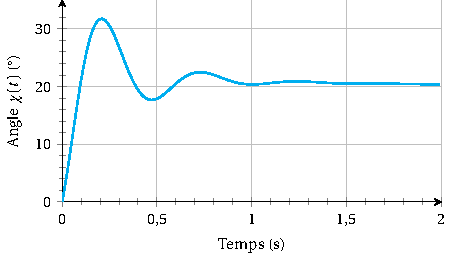
\includegraphics{\pathfig/systeme_corrige_reponse}
% \end{center}





%\begin{enumerate}[label=\arabic*),start=8]


\subparagraph{}\textit{Synthétiser la démarche d'étude et les résultats obtenus vis-à-vis du CDCF.}



%\end{enumerate}


%\end{conclusion}

\begin{center}

\includegraphics[width=.8\linewidth]{\pathfig/systeme_corrige_bode}

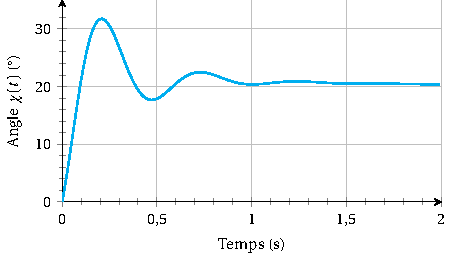
\includegraphics[width=.8\linewidth]{\pathfig/systeme_corrige_reponse}

%\begin{figure}[!ht]
%\centering
%\subfigure[Diagrammes de Bode de la FTBO.\label{calage_diag_bode_avance_phase}]{\includegraphics[width=0.45\linewidth]{\pathfig/systeme_corrige_bode}}\hfill
%\subfigure[Réponse en boucle fermée à un signal de consigne linéaire par morceaux.\label{calage_reponse}]{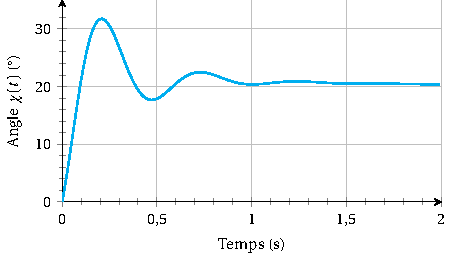
\includegraphics[width=0.45\linewidth]{\pathfig/systeme_corrige_reponse}
%}
%\captionof{figure}{Résultats pour un correcteur à avance de phase.
%\label{chap2:calage:resultats_avance_phase}}
%\end{figure}
%
\end{center}


\end{multicols}
\end{document}

\subparagraph{}\textit{}


\begin{center}
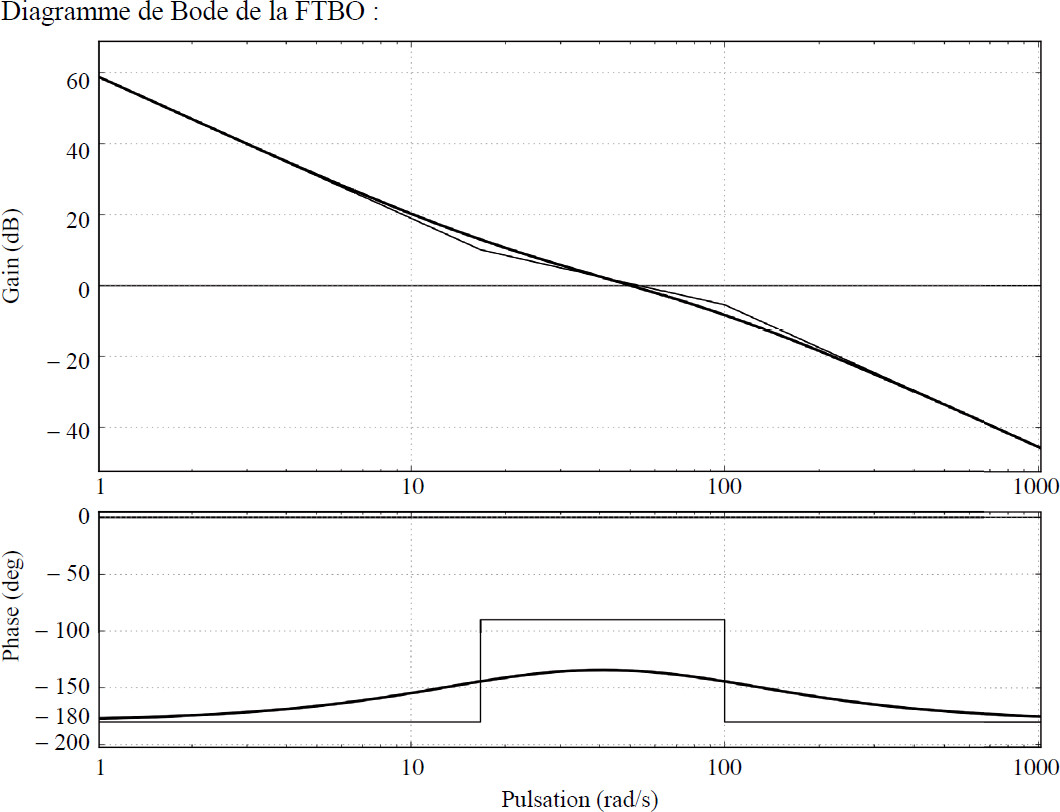
\includegraphics[width=\linewidth]{images/fig_06}
%\textit{}
\end{center}
\begin{center}
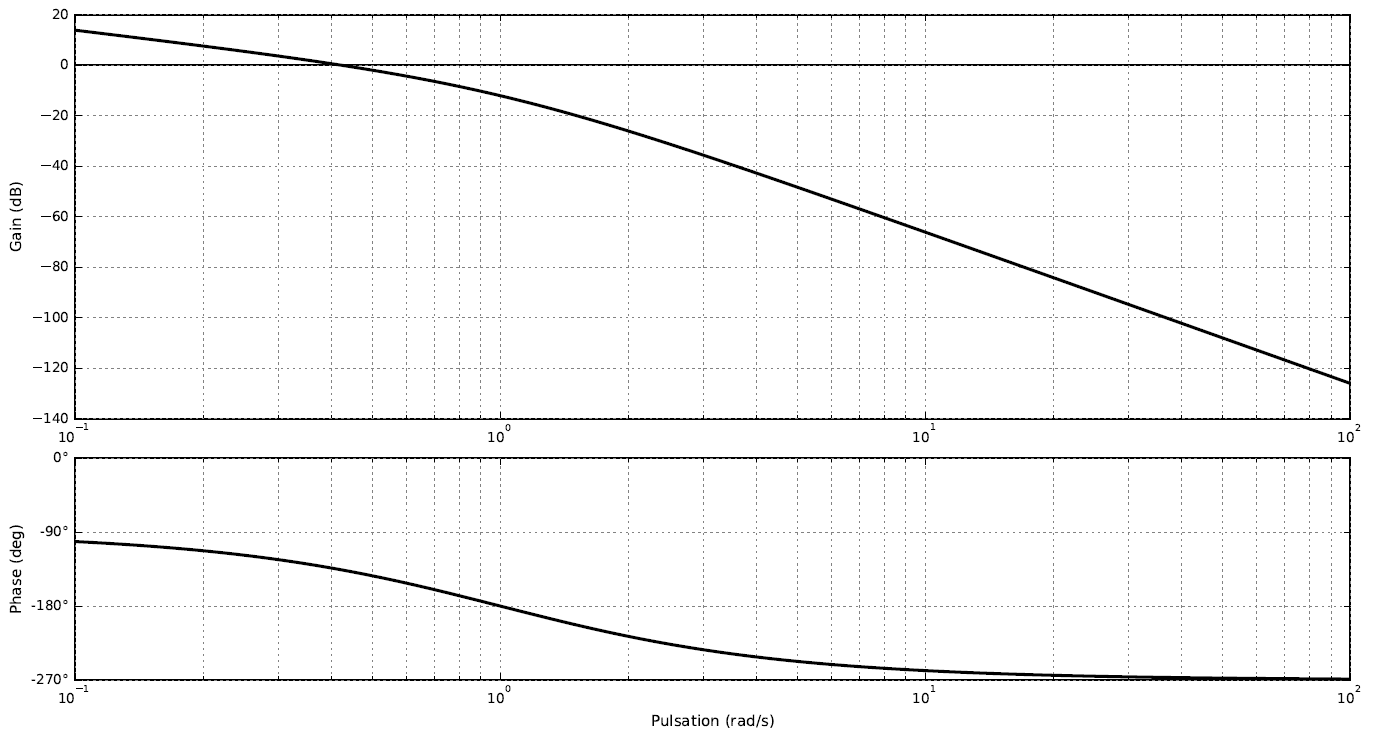
\includegraphics[width=\linewidth]{images/img_04}
%\textit{}
\end{center}




%%%%%%%%%%%%%%%%
%%%%%%%%%%%CORRECTION

\begin{questions}

\item Les conditions initiales sont supposées nulles. Dans le domaine de Laplace les équations deviennent : $Q(p) = S p X(p) + \dfrac{V}{B} p P(p)$ et $Mp^2 X(p) = S P(p) + F_{1\to 4}(p)$. On en déduit le schéma-blocs complété de la figure \ref{ex_calage_sb2_corr}.

\begin{figure}[!ht]
\centering

\scalebox{.65}{
\begin{tikzpicture}
\sbEntree{E1}
\sbBloc[4]{A}{$C$}{E1}
\sbComp[6]{C1}{A}
\sbBloc{B}{1}{C1}
\sbBloc[3]{C}{$K_e$}{B}
\sbBloc[3]{D}{$\dfrac{B}{Vp}$}{C}
\sbComp{C2}{D}
\sbBloc[3]{E}{$S$}{C2}
\sbSumh{C3}{E}
\sbBlocL{F}{$\dfrac{1}{Mp^2}$}{C3}
\sbBloc[3]{I}{$K_c$}{F}
\sbSortie[4]{S}{I}
\sbDecaleNoeudy[4]{C3}{G1}
\sbBlocr[0]{G}{$\dfrac{BS}{V}$}{G1}
\sbDecaleNoeudy[6]{Ddroite}{H1}
\sbBlocr[0]{H}{$C$}{H1}
\sbDecaleNoeudy[-4]{C3}{E2}

\sbRelier[$\Delta\theta_c(p)$]{E1}{A}
\sbRelier[$U_c(p)$]{A}{C1}
\sbRelier[$\varepsilon(p)$]{C1}{B}
\sbRelier[$I(p)$]{B}{C}
\sbRelier[$Q(p)$]{C}{D}
\sbRelier[]{D}{C2}
\sbRelier[$P(p)$]{C2}{E}
\sbRelier{E}{C3}
\sbRelier[$X(p)$]{F}{I}
\sbRelieryx{F-I}{G}
\sbRelierxy{G}{C2}
\sbRelier[$\Delta\theta(p)$]{I}{S}
\sbRelieryx{I-S}{H}
\sbRelierxy{H}{C1}
\sbRelier[]{E2}{C3}
\node[right] at(E2) {$F_{1\to 4}(p)$};
\end{tikzpicture}}

\captionof{figure}{Schéma-blocs avec fluide compressible.}
\label{ex_calage_sb2_corr}
\end{figure}

\item $X(p)={H}_{Q}(p)$.$Q(p)+{H}_{F}(p)$.${F}_{1 \rightarrow 4}(p).$

Analytiquement, il vient $ X(p) = \frac{1}{Mp^2}\left[F_{1\to 4}(p) + S\left( \frac{B}{Vp}Q(p) - \frac{BS}{V} X(p) \right)\right]$.\\
Donc $\left(Mp^2 +\frac{BS^2}{V}  \right) X(p) = F_{1\to 4}(p) +\frac{BS}{Vp}Q(p).$\\
D'où, $X(p)=\dfrac{BS}{Vp}\dfrac{1}{Mp^2 +\frac{BS^2}{V}} Q(p) + \dfrac{1}{Mp^2 +\frac{BS^2}{V}} F_{1\to 4}(p).$\\
Sous forme canonique : $X(p) = \dfrac{1}{p}\dfrac{1/S}{\frac{MV}{BS^2}p^2+1} Q(p) + \dfrac{\frac{V}{BS^2}}{\frac{MV}{BS^2}p^2+1}F_{1\to 4}(p)$.

On en déduit que ${H}_{Q}(p)= \dfrac{1}{p}\dfrac{1/S}{\frac{MV}{BS^2}p^2+1} = \dfrac{\num{1041.7}}{1+\num{1.7e-8}p^2}$, ainsi que :\\${H}_{F}(p)=\dfrac{\frac{V}{BS^2}}{\frac{MV}{BS^2}p^2+1} = \dfrac{\num{3.5e-8}}{1+\num{1.7e-8}p^2}$.

\item Avec deux pôles à partie réelle strictement positive, le système est instable. Ce modèle ne peut donc pas convenir.

%\item Le gain en décibel de la partie du second ordre a pour expression : $G_\textrm{dB}(\omega)=20\log\left(\dfrac{1}{\sqrt{\left(1-\dfrac{\omega^2}{\omega_Q^2}\right)^2+\dfrac{4\xi_Q^2\omega^2}{\omega_Q^2}}}\right)$\\
%La pulsation de résonance est $\omega=\omega_Q\sqrt{1-2\xi_Q^2}$ d'où le gain a la résonnance vaut $G_\textrm{dB}(\omega)=20\log\left(\dfrac{1}{2\xi_Q\sqrt{1-\xi_Q^2}}\right)$

%\item Modifier $\xi_Q$ revient à modifier en première approximation uniquement la valeur de la résonnance. Pour stabiliser le système, il faut que le gain en décibel soit nul pour $\omega_Q$. Pour cela, il faut diminuer la résonance de \SI{18}{dB}.

%Pour $\xi=\num{0.0001}$, le gain de la résonance est de \SI{74}{dB}. Il faut donc résoudre l'équation $20\log\left(\dfrac{1}{2\xi_Q\sqrt{1-\xi_Q^2}}\right)=74-18=\SI{56}{dB}$.

%Il s'agit d'une équation bicarrée dont la solution est $\xi_Q=\num{0.0008}$.

\item % En prenant $\xi_Q=\num{0.001}$, on assure une résonance encore plus faible de ce qui permet de s'écarter de la limite de stabilité.

Pour la marge de phase, d'après les diagrammes de Bode de la figure \ref{calagebode1}, on constate que le gain en décibel est nul pour $\omega=\SI{10}{rad.s^{-1}}$ et pour cette valeur la phase vaut \SI{-90}{\degree}, d'où une marge de phase de \SI{90}{\degree}.
On trouve bien une marge de phase supérieure à celle de \SI{50}{\degree} demandée dans le cahier des charges.
Le débit de fuite artificiel a permis de stabiliser le système.

\item On a $H_{BO2} (p)=\frac{K_e C K_c}{a_{1} p} \frac{1}{1+\frac{2\xi _{Q} }{\omega _{Q} } p+\frac{p^{2} }{\omega _{Q}^{2}}}$. Le pôle dominant est le pôle nul, on peut ainsi simplifier l'expression de la boucle ouverte par : $H_{BO2} (p)=\frac{K_e C K_c}{a_{1} p}$.

On en déduit que la bande passante vaut $\dfrac{K_c C K_e}{a_1} = \SI{12}{rad.s^{-1}}$.

\item L'erreur en réponse à un échelon serait nulle car la fonction de transfert en boucle ouverte est de classe 1. L'erreur en réponse à une rampe va tendre vers une valeur constante : $\dfrac{1}{K_{BO2}}=\dfrac{a_1}{K_eCK_c}=\dfrac{1}{12}=\num{0.083}.$


\item En ajoutant un correcteur intégrateur pur, l'erreur en réponse à une rampe serait bien nulle. En revanche, la fonction de transfert en boucle ouverte serait de classe 2 et conduirait donc à un système instable. Il convient d'utiliser un autre correcteur comme un correcteur à avance de phase.

\item Par mesure, la marge de phase semble être de \SI{50}{\degree} et la marge de gain de \SI{30}{dB}.

L'erreur pour des entrées de type rampe semble être nulle. 

Pour le critère de rapidité, on ne peut pas répondre avec la courbe proposée.

\medskip
La démarche de l'étude a consisté dans un premier temps à proposer un modèle simplifié du vérin hydraulique. \\Ce modèle étant instable, la prise en compte d'un débit de fuite dans le modèle a permis de le stabiliser. \\
Le modèle retenu a ensuite été analysé et il a permis de montrer que le système n'était pas suffisamment précis en réponse à une rampe. \\
L'analyse finale avec un correcteur à avance de phase a permis d'obtenir un modèle qui respecte le cahier des charges.

\end{questions}
\end{correction}



